\section{Unbalanced Classification}
\subsection{Binary genre classification: Rock - Jazz}
For this task we used the following features(
\textit{acousticness, danceability, energy, instrumentalness, liveness, speechiness, tempo, valence, duration and bit\_rate}). The dataset has 4,133 tracks. The class distribution is very unbalanced, with the minority class covering only 5.83\% of the data.
We evaluated the performance of the classifier on the validation set using first all features and then techniques for features compression/reduction such as PCA, and a sequential feature elimination. 
In the next section we will include only the best results. 
\subsubsection{Decision Tree}
We encoded the labels Rock and Jazz in binary values and we split the data into training set (70\%) and test set (30\%). We hyper-tuned the parameters of the model by testing 300 models obtained through a randomized grid search in a combination with a 5 fold cross validation. The model with the highest performance was the one without feature reduction. We noticed that PCA decreased substantially the performance of the class Jazz (f1-score = 0.18, recall = 0.11) except for the precision which was higher (0.58) compared to model exploiting all features.
In Table 2.1 we show the classification report. We see how even though the accuracy is 92\%, given the high unbalancing among classes, this estimate is not a good indicator of the real performance of the classifier, hence we focused exclusively on the f1 score of the minority class (which we tried to improve after detecting anomalies and balancing the data). The feature importance of the model instead, revealed that the most import feature is "\textit{energy}". The result is coherent with what are the main differences between genres, being Rock more energetic than Jazz on a musical level. 

\begin{figure}[!htb]
   \begin{minipage}{0.56\textwidth}
     \begin{tabular}{ccccc}
     \hline
     \textbf{Class} & \textbf{Precision} & \textbf{Recall} & \textbf{f1 score} & \textbf{Support} \\ \hline
     Jazz          & 0.35               & 0.24            & 0.28        & 72             \\ \hline
     Rock            & 0.95               & 0.97            & 0.96        & 1168            
     \end{tabular}
     \caption{Classification Report Unbalanced Decision Tree. The tree was constructed with criterion= entropy,max\_depth=6, min\_samples\_leaf= 5 and min\_samples\_split=10.\\ Accuracy = 92\%.}
     \label{Classification report: Test set Ripper}
   \end{minipage}\hfill
   \begin{minipage}{0.42\textwidth}
     \centering
     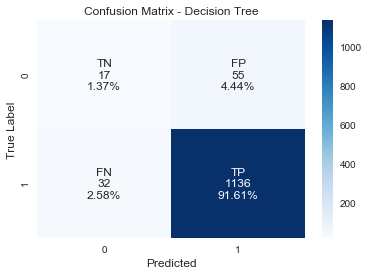
\includegraphics[width=0.7\linewidth]{images/cfm-unbalanced-decisiontree.png}
     \caption{Confusion Matrix Decision Tree. AUC score is 78.8\%}\label{Fig:Data2}
   \end{minipage}
\end{figure}

\subsubsection{K-Nearest Neighbor}
The best KNN model, was constructed with PCA features reduction (7 principal components explaining 90\% of the variance were selected). The attributes were normalized before being given in input to the PCA and ultimately to the model. The optimal number of neighbors is 8, while the metric used is the Manhattan distance. In Figure 2.3 and 2.4 we show the results. We noticed that the model constructed without PCA, had a lower f1 score (0.27) and recall (0.18) for the minority class. Overall, reducing the features improved the ability of KNN of recognizing Jazz songs, even though in terms of recall, the performance are far worst than those of the decision tree. 

\begin{figure}[!htb]
   \begin{minipage}{0.56\textwidth}
     \begin{tabular}{ccccc}
     \hline
     \textbf{Class} & \textbf{Precision} & \textbf{Recall} & \textbf{f1 score} & \textbf{Support} \\ \hline
     Jazz          & 0.57               & 0.18            & 0.27        & 72             \\ \hline
     Rock            & 0.95               & 0.99            & 0.97        & 1168            
     \end{tabular}
     \caption{Classification Report Unbalanced KNN (PCA) .\\Accuracy = 94\%.}
     \label{Classification report: Test set Ripper}
   \end{minipage}\hfill
   \begin{minipage}{0.42\textwidth}
     \centering
     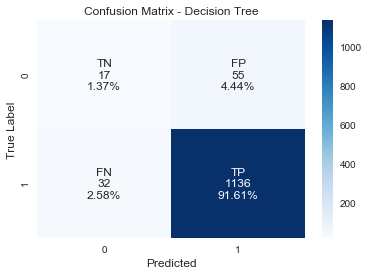
\includegraphics[width=0.7\linewidth]{images/cfm-unbalanced-decisiontree.png}
     \caption{Confusion Matrix KNN (PCA). AUC score is 78.1\%. }\label{Fig:Data2}
   \end{minipage}
\end{figure}


\subsection{Additional classification tasks}
\subsubsection{Song popularity classification}
We constructed a model able to predict whether a song is popular or not. The labels were generated using the information provided by the features \textit{"song\_hotness"} and \textit{"artist\_hotness"}. Our reasoning is based on the fact that songs sung by known artists that hit the top of the chart, should be considered popular. Songs for which these two features were respectively $>$ 0.15 and $>$ 0.4 were labeled as popular. The thresholds were decided after inspecting the mean and the scatter-plot of the above mentioned features.
Using the same dataset employed for for Decision Tree and KNN, we obtained 12,399 not popular (94.44\%) and 730 popular songs (5.56\%).
The task resulted very difficult to be solved. In fact the recall for class popular was extremely low (as shown in Table 2.1)

\begin{table}[h]
\centering
\begin{tabular}{ccccc}
\hline
\textbf{Class}       & \textbf{Precision} & \textbf{Recall} & \textbf{f1 score} & \textbf{Support} \\ \hline
\textbf{Not Popular} & 0.10               & 0.02            & 0.03              & 219              \\ \hline
\textbf{Popular}     & 0.94               & 0.99            & 0.97              & 3720             \\ \hline
\end{tabular}
\caption{Classification Report Decision Tree - Song popularity}
\label{Classification Report Decision Tree}
\end{table}

\subsubsection{Multi-genre classification \& Years of Rock}
We constructed a Decision Tree and a KNN to solve also these additional tasks. For the task Years of Rock we built a model able to predict the year of a given Rock song, while the multi-genre classificator, is able to classify tracks into 8 top genres ("Rock”, ”Pop”, ”Classical”, ”Hip-Hop”, ”Jazz”, ”Electronic”, ”Historical” and ”Folk"). The multi-genre classifier performed discretely, even though classes such as Pop and Jazz (which were the ones with less data) were not detected by neither Decision Tree and KNN (the recall was approximately 0.01). The classifier for classifying the year of Rock songs had good performances in terms of recall. For pages constraint the results will not be discussed in this report at a deeper level. 

\section{Anomaly Detection}
In this section we employed 7 different outlier detection algorithms. Since we didn't want to rely on just one method, we constructed an ensemble which provided us a more accurate outlier labelling (using majority voting). 
The analysis presented is conducted on the dataset used for the classification of Jazz and Rock (10 numerical features: \textit{Acusticness, Danceability, Energy, Instrumentalness, Liveness, Speechiness, Valence, Tempo} and \textit{Duration}) . Although we experimented also with other datasets and tasks (i.e. multi-genre classification and songs' emotion recognition) we decided to show the results of the classifier analysed in the previous section, as we wanted to improve its performance.
The outlier detection algorithms were selected after carefully analysing the distribution of our data, as we didn't want to use an algorithm that wouldn't be suitable for the task at hand.
The methods adopted for detecting the outlierness in the data, are: \textbf{DBSCAN, LOF, KNN, ABOD, AutoEncoder, Isolation Forest} and \textbf{Extended Isolation Forest}. 
The results of the last two were compared, because we wanted to observe if there were any differences in the scoring. Considering that the scores were very similar, in a majority voting system we decided that employing both of them would have been redundant, hence among the 2 we selected the Extended Isolation Forest.
We fist analysed each feature individually using box-plots and then we calculated the \textbf{IQR} scores.\\In Figure 2.5 we can observe that outliers are found in \textit{danceability, liveness, speechiness, tempo, duration} and \textit{bit rate}. 
We noticed that few tracks have a duration that exceeds 3,033 sec. This value is extremely high compared to the mean duration of Rock and Jazz songs, which is respectively 237 sec and 379 sec. One explanation is that some tracks were recorded during live concerts. \\We also noticed few abnormal values of bit rate. After some research we discovered that music extracted from video has higher bit rate compared to mp3 tracks, hence we deduced that some of the tracks were extracted from video-recording. In Table 2.2 instead, we show the results of the IQR method. The IQR highlighted more outliers than the amount we wanted to remove. Furthermore, the IQR considers each feature individually, hence it cannot judge the outlierness of a record in the full context.

\begin{figure}[!htb]
  \centering
  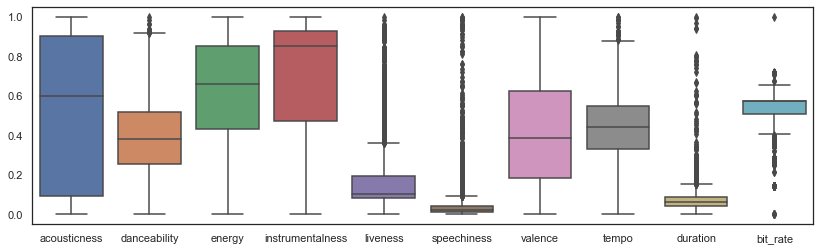
\includegraphics[width=0.7\linewidth]{images/normalized-boxplots-echonest_AD.png}
  \caption{Normalized box-plots for outliers' visualization}
\end{figure} 

\begin{table}[!htb]
\centering
\begin{tabular}{lllllll}
\hline
\textbf{Attributes} & \textbf{Q1} & \textbf{Q2} & \textbf{IQR} & \textbf{\begin{tabular}[c]{@{}l@{}}Lower \\ Whisker\end{tabular}} & \textbf{\begin{tabular}[c]{@{}l@{}}Upper\\ Whisker\end{tabular}} & \textbf{\begin{tabular}[c]{@{}l@{}}Potential\\ Outliers\end{tabular}} \\ \hline
danceability       & 0.271       & 0.501       & 0.229        & -0.072                                                            & 0.845                                                            & 11                                                                    \\ \hline
liveness           & 0.104       & 0.209       & 0.104        & -0.053                                                            & 0.366                                                            & 413                                                                   \\ \hline
speechiness        & 0.035       & 0.065       & 0.029        & -0.008                                                            & 0.109                                                            & 409                                                                   \\ \hline
tempo              & 101.7       & 150.2       & 48.5         & 29.03                                                             & 223.04                                                           & 21                                                                    \\ \hline
bit\_rate          & 226         & 256         & 30           & 181                                                               & 301                                                              & 1182                                                                  \\ \hline
duration           & 147         & 280         & 133          & -52.5                                                             & 479.5                                                            & 226                                                                   \\ \hline
\end{tabular}
\caption{IQR scores per features}
\label{IQR scores for features not normalized}
\end{table}

\subsection{Methodology and Results}
Before removing the outliers, our dataset consisted of 4,133 records and 10 attributes. Considering that some of the algorithms adopts metrics meaningless in high dimensions, we tested their performance on both PCA projection and fully-dimensional dataset. To our surprise methods such as DBSCAN and KNN detected almost the same records regardless of the dimension's size. We concluded that 10 features didn't impact much on the goodness of the estimation, hence we performed the whole analysis without reducing the features.\\After inspecting the distribution of our data, we focused on identifying the top 1\% outliers. In order to do so, we used a contamination parameter to instruct the algorithms in identifying only the specified portion of anomalies. However, other methods such as DBSCAN and KNN were not provided with this option, therefore an hyper-parameter tuning was needed until the right configuration was found. The right setting for DBSCAN was identified with epsilon = 3.0 and min\_sample = 15. We noticed that as we reduced the radius, the majority of the data were incorrectly labeled as outliers. KNN instead, performed best with the number of neighbors set to 50. \\Majority of the samples labeled as outlier by LOF were perfectly matching those detected by the previous two methods. This was interpreted as an indicator that the chosen settings were optimal. ABOD however, was the only algorithm which labeled as inlier some records which were considered as outlier by the majority. 
We also tested the Isolation Forest (comparing the versions of sklearn and eif repository) and the Extended Isolation Forest. The forest was built using 300 classifiers with a sample size of 256. These algorithms, didn't provide an outlier label. Hence, we had to fix a threshold in order to label the data. After inspecting the histogram of the outlier scores, we decided to set the threshold to 0.60. The cut-off choice was crucial, as the majority of the data was attributed a score between 0.45 and 0.55, and no records had a score higher than 0.70. Using a threshold equal to 0.50 would have significantly increased the number of detection. 
Even with this threshold, compared to others, these approaches doubled the number of outliers detected.  
We noticed that Extended and Standard Isolation Forest performed similarly. We also experimented with AutoEncoders for detecting anomalies. We opted for an under-complete AutoEncoder with a bottle-neck of 3 neurons. The model was trained using the ReLU activtion function over 400 epochs. Finally, the outcome of model, was in line with the detections made by the previously described methods. \\ 
\begin{figure}[!htb]
  \centering
  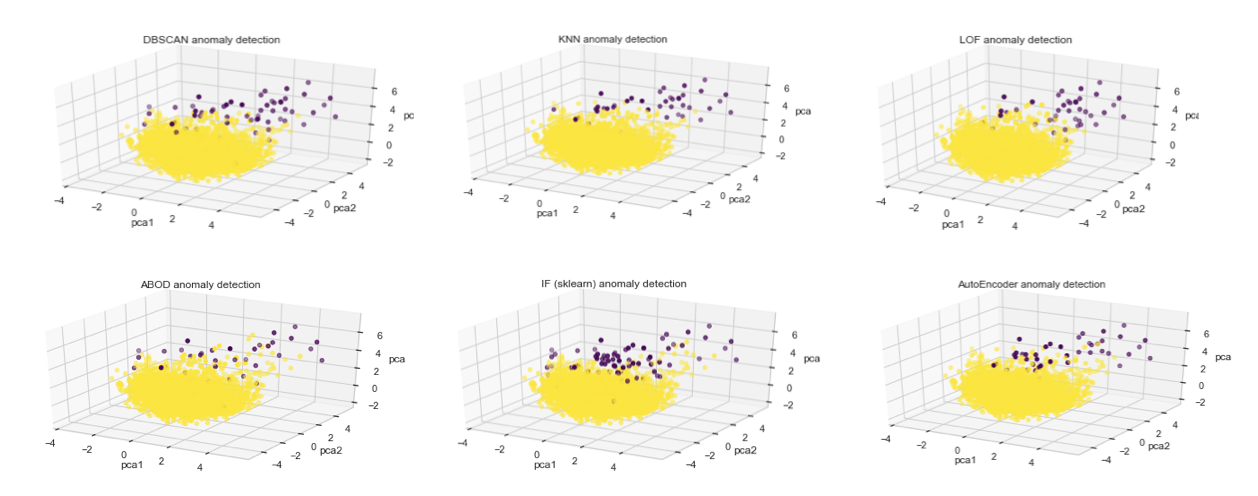
\includegraphics[width=1\linewidth]{images/anomaly-detection_scatters.png}
  \caption{Scatter plots of anomaly detection methods. From left to right: DBSCAN, KNN, LOF, ABOD, Isolation Forest and AutoEncoder. In yellow are represented inliers, whereas in purple are indicated the outliers. The PCA representation is used for plotting the data in 3 dimensions. The anomalies represent the top 1\% outliers.}
\end{figure}


\begin{table}[!htb]
\centering
\begin{tabular}{llllllll}
\hline
                             & DBSCAN                 & KNN                    & LOF                    & IF                     & EIF                    & ABOD                   & AutoEncoder            \\ \hline
\multicolumn{1}{c}{outliers} & \multicolumn{1}{c}{62} & \multicolumn{1}{c}{40} & \multicolumn{1}{c}{42} & \multicolumn{1}{c}{62} & \multicolumn{1}{c}{61} & \multicolumn{1}{c}{41} & \multicolumn{1}{c}{42} \\ \hline
\end{tabular}
\caption{Number of outliers detected by each method.}
\label{Number of outliers detected by each method}
\end{table}


\subsection{Majority Voting}

The final outcome of the anomaly detection was obtained through a majority voting schema. After evaluating the proposed methods, we assigned a label to each row of the dataset, indicating if the track was an outlier or not. The ensemble of anomaly detection methods, assigned the outlier label to a track, only if the majority of its constituent agreed with that assignment. This approach identified 38 outliers in total. 
After inspecting the scatter-plots of each pairs of attributes, we noticed that visible outliers were correctly detected (for some combination of features), as it can be observed in Figure 2.7. 
It is clear that the attribute \textit{"duration"} is the one that in combination with other features, generated isolated points.
In Figure 2.8 instead, we show a 3D representation of the data, with the labelling assigned by the ensemble of outliers algorithms.
\begin{figure}[!htb]
  \centering
  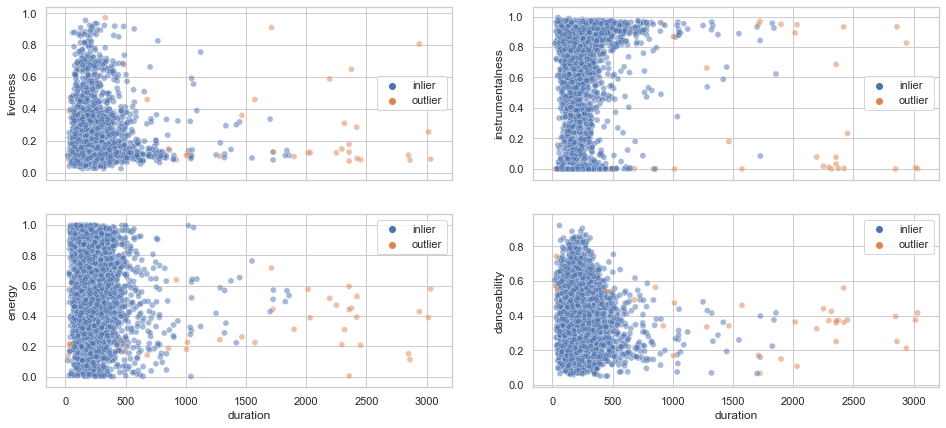
\includegraphics[width=0.85\linewidth]{images/4scatter-anomaly_winner.png}
  \caption{Top 1\% anomalies on 4 pairs of attributes, with majority voting.}
 \end{figure} 

\begin{figure}[!htb]
  \centering 
  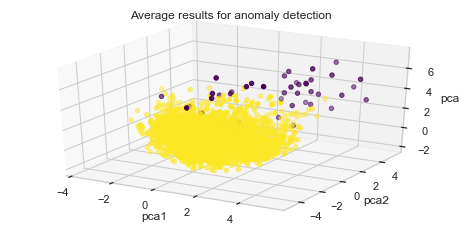
\includegraphics[width=0.37\linewidth]{images/winner-outliers.png}
  \caption{Scatter plot of Top 1\% outliers detected using majority voting.}
\end{figure}
\newpage
\section{Imbalanced Learning}
\textbf{Binary genre classification: Rock - Jazz}\\
In this section we applied several balancing technique on the dataset used for classifying Jazz and Rock songs. The data under analysis do not contains outliers (as they were removed in the previous section). 
We trained a Decision tree and KNN classifier, with the aim of improving the f1 score of the minority class (Jazz). We focused on this metric as we wanted to find a good trade-off between precision and recall, and make our model able to learn and classify correctly Jazz songs, without penalizing the performance on class Rock. The dataset is composed by 4,095 tracks and 10 attributes.  
Below we show the data distribution and unbalancing percentages.

\begin{figure}[!htb]
  \centering 
  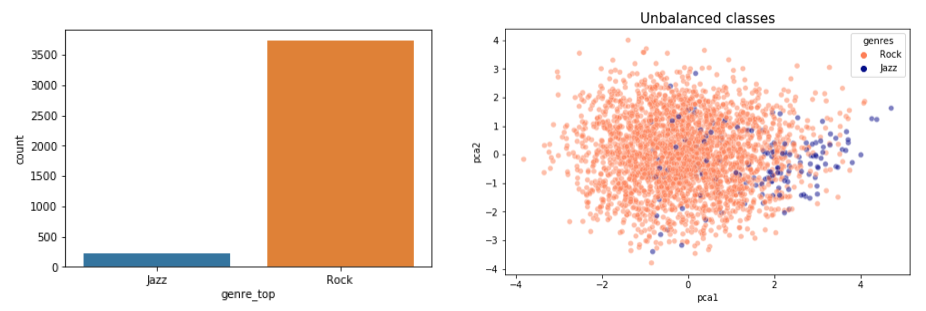
\includegraphics[width=0.72\linewidth]{images/countplot-scatter_Jazz-Rock.png}
  \caption{Count-plot and scatter-plot of the class distribution (94.33\% Rock - 5.67\% Jazz).}
\end{figure}

We experimented with the following algorithms: \textbf{Random Undersampling}, \textbf{Condensed-NN}, \textbf{Tomek's Link}, \textbf{Random Oversampling}, \textbf{SMOTE} and \textbf{ADASYN}. The SMOTE algorithm was also compared with the \textbf{K-Means SMOTE}. The latter improves the performance of the standard SMOTE algorithm. This is due to the fact that K-Means SMOTE groups the data into micro-clusters before generating synthetic data. This avoids that data are over-sampled in area in which there are noise points. In Figure 2.10 we show the differences between the two methods. We can observe that K-Means SMOTE is more efficient than SMOTE in identifying the area in which the minority class in located (and more concentrated).
It is important to mention that all balancing approaches, were applied exclusively on the training data. In addition to that, since we didn't want to bias our classifiers with the hyper-parameters discovered in an unbalanced setting, we performed a random search to fine-tune the Decision trees and KNNs. 

\begin{figure}[!htb]
  \centering 
  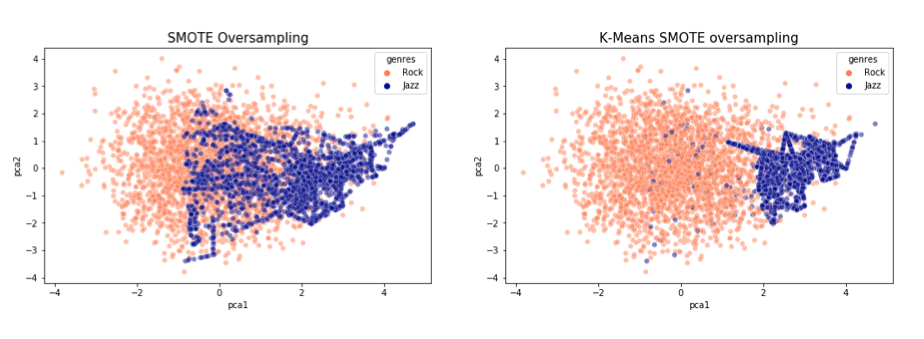
\includegraphics[width=0.75\linewidth]{images/SMOTE_KSMOTE.png}
  \caption{SMOTE and K-Means SMOTE oversampling.}
\end{figure}

\subsubsection{Decision Tree}

The model with the highest performance in terms of f1 score is K-Means SMOTE, whose score is 40\% (+12\% w.r.t. the unbalanced dataset). We noticed that this algorithm, improved also the precision of class Jazz(45\%). Instead, if we focus exclusively on the recall, we can see that random undersampling identifies 90\% of the Jazz tracks on the test set. However the high recall, it's paid at the expense of an high false negative rate. In fact, the precision of class Jazz is decreased to 13\% as well as the recall of class Rock which is 63\% (was 98\% on the unbalanced dataset). In Table 2.4 we compare the classification report of K-Means SMOTE and the decision tree with unbalanced classes, while in Figure 2.11 we summarize the scores obtained by each balancing technique on the minority class Jazz.

% Classification report: Unbalanced vs K-Means SMOTE
\begin{table}[!htb]
\centering
\begin{tabular}{cccc
>{\columncolor[HTML]{C0C0C0}}c cccc}
\hline
\multicolumn{1}{l}{} & \multicolumn{3}{c}{\textbf{Unbalanced}}                  & \textbf{} & \multicolumn{3}{c}{\textbf{K-Means SMOTE}}               & \multicolumn{1}{l}{} \\ \hline
\textbf{Class}       & \textbf{Precision} & \textbf{Recall} & \textbf{f1 score} &           & \textbf{Precision} & \textbf{Recall} & \textbf{f1 score} & \textbf{Support}     \\ \hline
\textbf{Jazz}        & 0.39               & 0.21            & 0.28              &           & 0.45               & 0.36            & 0.40              & 70                   \\ \hline
\textbf{Rock}        & 0.95               & 0.98            & 0.97              &           & 0.96               & 0.97            & 0.97              & 1159                 \\ \hline
\end{tabular}
\caption{Classification Report: Unbalanced and K-Means SMOTE. The Unbalanced decision tree has depth = 8 using Gini index for splitting nodes, while the balanced decision tree has depth = 9 and utilized the Entropy.}
\label{Classification Report: Unbalanced and K-Means SMOTE}
\end{table}


\begin{figure}[!htb]
  \centering 
  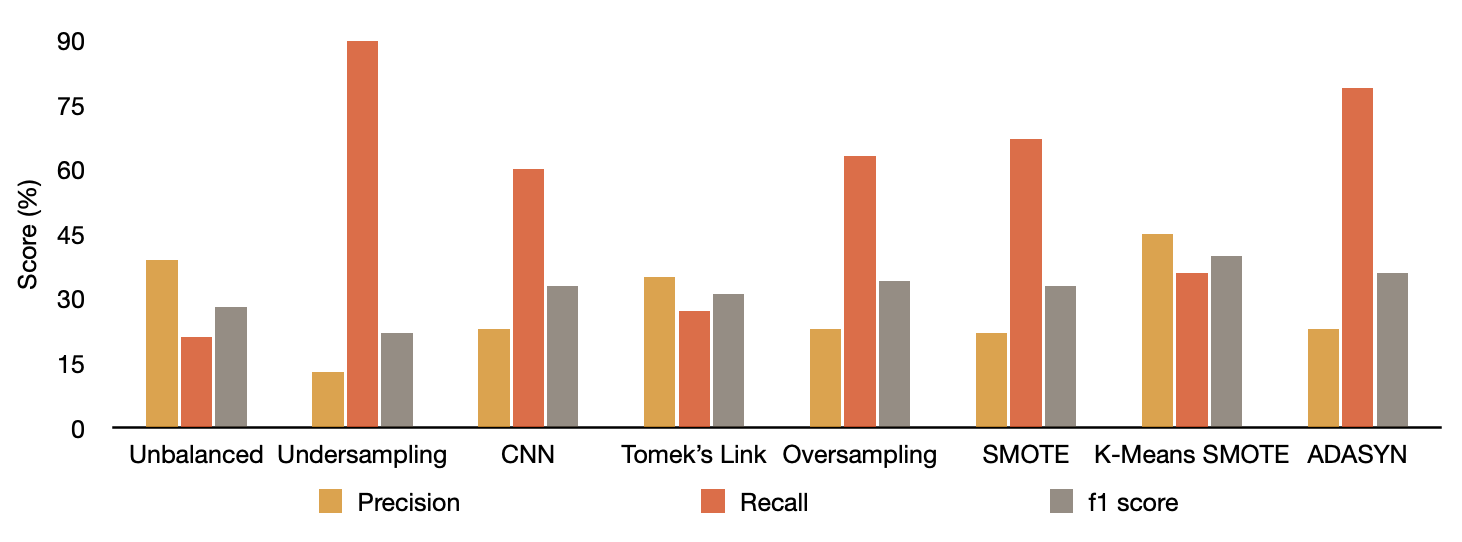
\includegraphics[width=0.7\linewidth]{images/imb-learn_scores-classifiers.png}
  \caption{Decision Tree scores for each imbalanced learning method. The metrics refers to the minority class Jazz.}
\end{figure}


\subsubsection{K-Nearest Neighbor}
The highest f1 score is provided by undersampling (0.46). Good performance were obtained also using CNN and Tomek's Link (f1 score is 0.40 and 0.38 respectively).
In terms of recall of the minority class, the best balancing technique is still undersampling, which increased the recall from 0.27 to 0.73. Although the precision decreases from 0.53 to 0.34, we observe that it didn't affect the ability of the classifier to recognize Rock songs with high precision and recall (for these the precision increased of +0.07 while the recall decreased from 0.99 to 0.91). 
In terms of precision, CNN outperformed the others, with a score of 0.60. However when using this method, the recall of the minority class has only a slight improvement (+0.03). 
In conclusion, undersampling resulted to be the best balancing algorithm for classifying Rock and Jazz songs using KNN.

\begin{table}[!htb]
\centering
\begin{tabular}{cccc
>{\columncolor[HTML]{C0C0C0}}c cccc}
\hline
\multicolumn{1}{l}{} & \multicolumn{3}{c}{\textbf{Unbalanced}}                  & \textbf{} & \multicolumn{3}{c}{\textbf{Random Undersampling}}        & \multicolumn{1}{l}{} \\ \hline
\textbf{Class}       & \textbf{Precision} & \textbf{Recall} & \textbf{f1 score} &           & \textbf{Precision} & \textbf{Recall} & \textbf{f1 score} & \textbf{Support}     \\ \hline
\textbf{Jazz}        & 0.53               & 0.27            & 0.36              &           & 0.34               & 0.73            & 0.46              & 70                   \\ \hline
\textbf{Rock}        & 0.96               & 0.99            & 0.97              &           & 0.98               & 0.91            & 0.95              & 1159                 \\ \hline
\end{tabular}
\caption{Classification Report KNN: Unbalanced and Random Undersampling}
\label{Classification Report KNN: Unbalanced and Random Undersampling}
\end{table}

\begin{figure}[!htb]
  \centering 
  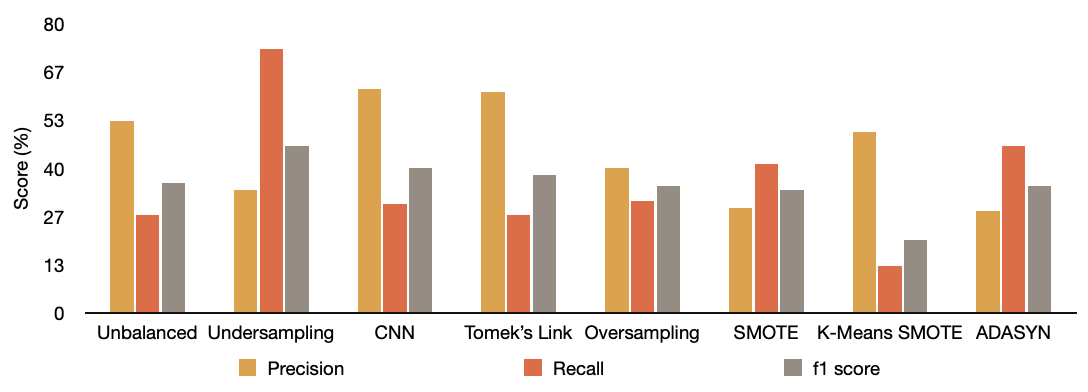
\includegraphics[width=0.7\linewidth]{images/imb-lean_score-classifiers-KNN.png}
  \caption{KNN scores for each imbalanced learning method. The metrics refers to the minority class Jazz }
\end{figure}
\newpage
\subsection{Comparing Decision Tree and KNN}
\textbf{Decision Tree:}
Although K-Means SMOTE has the highest f1-score, the best AUC score is obtained using ADAYSN (0.85). The unbalanced classifier has the lowest AUC (0.781). Furthermore, all balancing approaches increased this metric of at least +0.5, except for Random Oversampling which did not prove to be very effective provided the AUC similar to the unbalanced one.\\
\textbf{KNN:} The highest AUC score is obtained by the undersampling approach, which proved to be very effective for this task. Similar results are provided by Tomek's Link which has an AUC score of 0.888.
\\
In conclusion for solving the binary classification task Rock-Jazz the KNN classifier with random undersampling provides higher performance compared to the other.

\begin{figure}[h]
  \centering 
  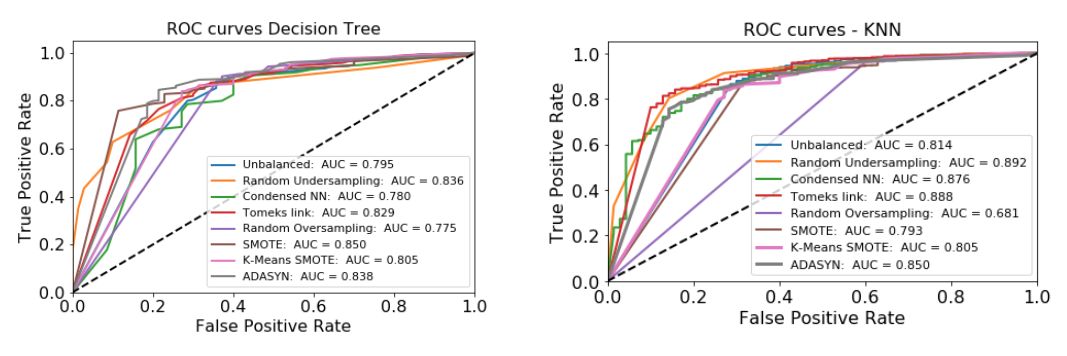
\includegraphics[width=0.95\linewidth]{images/imb-learn_roc-curves_DT-KNN.png}
  \caption{ROC curves of balancing techniques for Decision Tree and KNN.}
\end{figure}

\subsection{Additional classification tasks}
\subsubsection{Song Popularity classification}
The highly unbalanced task of song popularity classification, resulted to be quite difficult to be solved. The classes were extremely skewed with 12,399 not popular songs (94.44\%) and 730 popular songs (5.56\%). The minority class scores for the unbalanced Decision Tree classifier are: recall = 0.01, precision = 0.10 and f1-score = 0.02. In this task we focused exclusively on the recall, as we wanted our model to be able to detect as many popular song as possible. The best method resulted to be SMOTE which boosted the recall up to 0.67.  
\subsubsection{Multi-genre classification}
For this task we tried to improve the multi-genre classification of the following 8 genres: Rock, Pop, Classical, Jazz, Historical, Electronical, Hip-Hop and Folk. Genres like Pop and Jazz represented around 5\% and 1\% of the whole dataset, and for this reason the classifier was not able to detect them (in fact the recall was these classes did not exceed 0.05). Jazz and Pop had an f1 score of 0.08 and 0.04, which we were able to improved to 0.16 using SMOTE oversampling.